\documentclass[10pt, a4paper]{article}
\usepackage[ngerman]{babel}
\usepackage[utf8]{inputenc}
\usepackage[T1]{fontenc}
\usepackage{color}
\usepackage{hyperref}
\usepackage{comment}
\usepackage[backend=biber,style=alphabetic,]{biblatex}
\usepackage{graphicx}
\usepackage{wrapfig}
\usepackage{caption}
\DeclareCaptionFormat{citation}{%
   \ifx\captioncitation\relax\relax\else
     \captioncitation\par
   \fi
   #1#2#3\par}
\newcommand*\setcaptioncitation[1]{\def\captioncitation{\textit{Source:}~#1}}
\let\captioncitation\relax
\captionsetup{format=citation,justification=centering}
\graphicspath{ {./images/} }

\addbibresource{literature.bib}

\title{Projektbreicht Smart Music Player}
\author{Anton Bracke\\Jan Eberlein\\Tom Calvin Haak\\Julian Hahn\\Nick Loewecke}

\begin{document}
\maketitle
\newpage
\tableofcontents
\newpage

\section{Einleitung}
Ein zentraler Teil des Studiengangs \glqq Informationstechnologien\grqq{} ist es, Softwareentwicklung in Teams und Kommunikation mit Kund:innen zu erlernen. \cite{Qualifikationsziele_Informationstechnologien}
Dies passiert vor allem im Modul \glqq Projekt Informatik (PROI)\grqq{}.
In diesem arbeiten Studierende ein Semester lang in kleinen Gruppen an verschiedenen Projekten.
Diese bilden häufig reale Sachverhalte der Softwareentwicklung ab und werden meist von Firmenpartner:innen aus der Wirtschaft gestellt.
Die Teams wählen ein oder mehrere Projekte, die sie gerne bearbeiten würden, und stellen sich mit einer Kurzbewerbung bei den entsprechenden Firmen vor.
Welche Teams die jeweiligen Projekte bearbeiten, entscheiden die Firmen selbst.
\\
Dieser Bericht beschreibt das Projekt und dessen Verlauf, dass das Autoren-Team für die macio GmbH aus Kiel bearbeitete.

\subsection{Unternehmen}
\colorbox{red}{TODO:}was macht macio aus
\subsection{Projektidee}
Im Rahmen des Projekt Informatik möchte Macio ihr Portfolio im IoT-Bereich erweitern, sowie ihren Empfangsraum im Standort Kiel verschönern.
Hierfür soll eine smarte Spielzeug-Box gebaut werden.
Smarte Spielzeuge gibt es im kommerziellen Bereich viele, daher soll dieses Projekt eine Open-Source-Alternative schaffen.\\
Genauer handelt es sich um eine Musik-Box, die NFC-Chips lesen und Spotify Connect unterstützen soll.
Auf die Box können dann Spielzeuge (z.B. in Form von kleinen Figuren) mit integrierten NFC-Chips gestellt werden, um spezifische Musik abspielen zu lassen.
Die Musik wird von Spotify-Connect über eine bereits bestehende Musik-Anlage abgespielt.
Falls es im Rahmen des Projektes möglich ist, sollen die Nutzer in der Lage sein, zwischen verschiedenen Musikanbietern zu wechseln.
NFC-Chips und die zugehörige Musik sollen über ein Web-basierte Benutzeroberfläche konfiguriert werden können.
Diese Benutzeroberfläche soll von der Box ausgeliefert und primär für Smartphone-Bedienung gestaltet werden.
Da es sich um ein Open Source Projekt mit entsprechender Lizenz handelt, muss auch eine aussagekräftige, öffentliche Dokumentation verfasst werden.
Macio stellt die benötigte Hardware zur Verfügung und unterstützt bei technischen Fragen.

\subsubsection{Minimal Requirements}
\begin{enumerate}
  \item NFC-Tags lesen, schreiben und entschlüsseln
  \item Mit Spotify Connect verbinden und arbeiten
  \item Responsive UI konzeptionieren und umsetzen
  \item Aussagekräftige Dokumentation mit Benutzerhandbuch
\end{enumerate}
\subsubsection{Stretch Goals}
\begin{enumerate}
  \item Sound Wiedergabe auf der Box selbst
  \item Unterstützung anderer Musikdienste / Plugin-Subsystem
  \item 3D-Modellierung und Print einer passenden Box
  \item Cloud-Anbindung der Box, Auslieferung des UI aus der Cloud
\end{enumerate}

\section{Projektplanung}

\subsection{Projekt Management}
\colorbox{red}{TODO:}ticket pool in github, gemeinsame Absprache (im team und mit Kunden) was in den aktuellen Milestone kommen soll, alles zentral, 3x daily standup, gemeinsamer google calendar, gemeinsamer Discord Server (für spontaneres und informelleres gemeinsames Arbeiten), interne team evaluation und regelmäßiges feedback

\subsection{Projektrisiken}
\colorbox{red}{TODO:}Welche Riskiken hatten wir + Risikomatrix? lohnt sich dieser Abschnitt?

\subsection{Phasenplanung}
\subsubsection{Projektstartphase}
\colorbox{red}{TODO:}Github aufsetzen, Tickets befüllen, Anforderungen verstehen, Team einarbeiten in Technologien

\subsubsection{Realisierungsphase}
\colorbox{red}{TODO:}Iteratives Arbeiten in Meilensteinen/Sprint mit Länge ca. 2 Wochen. Coden etc. Jedes Arbeitspaket wird einzeln getestet und von mindestens zwei anderen Personen reviewt (Technische Funktionalität wird automatisch getestet)

\subsubsection{Vermarktungsphase}
\colorbox{red}{TODO:}Testsachen aus Code nehmen, Anleitung schreiben, Informationen veröffentlichen

\subsection{Projektstrukturplan}
\colorbox{red}{TODO:}einzelne subsubsections über frontend, backend, hardware, devops, und dann erklären was das beinhaltet?

\subsection{Beispielhafte Arbeitspakete}
\colorbox{red}{TODO:}1-2-3 Beispielhafte Arbeitspakete ausarbeiten? Am besten auch welche, die von anderen abhängig

\subsection{Netzplan}
\colorbox{red}{TODO:}wie hängt alles zusammen mit approx Zeit, wobei wir die Zeit vielleicht weglassen?

\section{Machbarkeitsstudie}

\subsection{NFC Tag}
\subsubsection{lesen}
Um mit NFC Tags arbeiten zu können, müssen diese auch entschlüsselt bzw. gelesen werden können.
Hierfür ist ein Hardware NFC-Reader notwendig, der die Daten ausliest und an die Box kommuniziert.
Dieser emuliert dafür Keyboard Eingaben, die die Tag-IDs darstellen.
\textit{Evdev}, ein Kernel Modul von Linux, könnte dann zum Abgreifen dieser Keyboard-Eingaben genutzt werden. Mit \textit{node-evdev}\footnote{https://github.com/sdumetz/node-evdev} kann \textit{evdev} auch mit Node genutzt werden. Mit dem Fork\footnote{https://github.com/anbraten/node-evdev} von Anbraten wird zusätzlich der Raspberry Pi und die Typescript Unterstützung zur Verfügung gestellt.

\subsubsection{schreiben}
Ein NFC-Tag hat generell eine feste ID.
Um weitere Daten auf einen NFC-Tag schreiben zu können, benötigt der NFC-Tag also einen eigenen Speicher.
Ist dieser vorhanden, können dort z.b. Kontaktdaten hinterlegt werden. Werden diese dann von einem Smartphone gelesen, öffnet sich die Kontakte-App und der auf dem NFC-Tag gespeicherte Kontakt kann abgespeichert werden.
Dafür wäre einerseits ein spezieller NFC-Reader, der auch schreiben kann, sowie eine spezielle Library notwendig.

\subsection{Raspberri Pi}
\subsubsection{Docker Integration}
Auf einem Raspberri Pi Docker zu installieren und zum Laufen zu bringen wird in vielen Anleitungen online beschrieben\footnote{https://phoenixnap.com/kb/docker-on-raspberry-pi}.

\subsubsection{Öffentlich zugängliches Web Interface}
Auf einem Raspberri Pi könnte eine Web Anwendung gehosted werden, welche die allgemeine Web Anwendung für alle Boxen darstellen soll.
Um diese Web Anwendung von außerhalb des eigenen Netzwerkes erreichen zu können, muss innerhalb des Routers ein Port ge-forwarded werden.
Dann kann der Pi und dessen Webinterface unter der öffentlichen IP xxx.xxx.xxx.xxx des Routers erreicht werden.
Da sich die öffentliche IP-Adresse eines privaten Internet-Anschlusses in der Regel täglich ändert, wird zum einfachen finden der IP ein DynDns Service benötig, welcher eine feste Domain in die wechselnde IP Adresse des Routers übersetzt.
Alternativ ginge es auch ohne Port-Forwarding mit nginx und ngrok \footnote{https://vatsalyagoel.com/setting-up-a-public-web-server-using-a-raspberry-pi-3/}.
Für Unerfahrene wären diese notwendingen Schritte zu Beginn etwas komplexere Thematiken. Der effektive Arbeitsaufwand hängt daher auch sehr stark von der Erfahrung der einzelnen Teammitglieder ab.

\subsubsection{URL für UI festlegen}
Über ein mDNS Service, der auf dem Raspberri Pi läuft, wäre es möglich für die statische Public-IP eine eigene URL anzulegen.
Dafür sind verschiedene mDNS Services möglich, potentiell ist auch eine Domain notwendig.

\subsection{User Interface}
\subsubsection{Zugriff auf NFC Reader von Cloud Anwendung}
Um von der App auf die Daten vom NFC-Reader der verschiedenen Boxen zuzugreifen, wäre ein zentrales Backend mit einer API sinnvoll.
Der Computer der Box könnte beim Lesen eines NFC-Tag Daten über einen API Call an die Cloud Anwendung schicken, sodass die zusätzlich zu dem Backend verbundene App das gewünschte Event triggern kann.

\subsubsection{Login via Spotify, Youtube, etc.}
Es gibt ein Feathers Plugin, welches die Möglichkeit bietet OAuth Provider zu nutzen, um sich über andere Services wie Spotify anzumelden.

\subsubsection{Gleichen Nutzer bei verschiedenen Loginvarianten wiedererkennen}
Um gleiche Nutzer zu erkennen, müssten Merkmale angelegt werden, über die diese Nutzer wiedererkennbar wären.
Die E-Mail wäre hierbei ein geeignetes Merkmal, da dies einzigartig ist. Über gesetzte Scopes in der OAuth Anfrage kann diese vom jeweiligen Provider mitgeliefert werden.
Um die E-Mail als Wiedererkennungsmerkmal zu verwenden, muss vorausgesetzt sein, dass Nutzer immer die gleiche E-Mail bei den unterschiedlichen Providern nutzen. Dies ist aber nicht immer der Fall.
Daher könnte dem (bereits eingeloggten) Nutzer die Möglichkeit gegeben werden, weitere Accounts zu dem bestehenden hinzuzufügen und entsprechend in der Datenbank zu hinterlegen.

\subsubsection{Musik Artwork laden}
Sollte bei der Verwendung von Spotify kein Problem sein, da zu jeder Anfrage von Titeln oder Liedern auch eine Liste von Bildern enthalten ist.\footnote{https://stackoverflow.com/questions/10123804/retrieve-cover-artwork-using-spotify-api}

\subsubsection{Eigene Bilder hochladen}
Eigene Bilder hochzuladen sollte möglich sein. In unserem Kontext mit Vue.js und Node.js würde das Plugin \textit{vue-picture-input} helfen.
Mit einem Axios Post könnte das Bild an das Backend gesendet werden. \footnote{https://www.digitalocean.com/community/tutorials/vuejs-uploading-vue-picture-input}

\subsubsection{Spotify Connect Lautsprecher auswählen}
Das Auswählen von einem spezifischen Spotify Connect Lautsprecher ist möglich.
Über einen API Call an die Spotify API mit dem Endpunkt \textit{/v1""/me""/player""/device} wird eine Liste von allen verbundenen Geräten geliefert. Über den Endpunkt kann ein entsprechendes Lied zum Abspielen über den jeweiligen \textit{Spotify Connected Speaker} übergeben werden.
Sollte nicht explizit ein Lautsprecher angegeben werden, so wird der zuletzt aktive genutzt. Dieser hat bei \textit{is\_active} den Wert \textit{true}. \footnote{https://developer.spotify.com/documentation/web-api/guides/using-connect-web-api/}

\subsubsection{Spotify Connect Lautsprecher speichern}
Die Liste von verbundenen Geräten, die über einen Call an die Spotify API erhalten wird, enthält auch ein eindeutiges Feld \textit{id}, welches sich zusammen mit einem Namen speichern lässt.

\subsubsection{In der Cloud Anwendung die eigene Box auswählen / verbinden}
Bei der Ersteinrichtung könnte der Nutzer über die Eingabe der MAC Adresse oder über eine andere festgelegte ID die eigene Box finden und zu seinem Account hinzufügen. Die jeweilige Box wäre dem System anschließend bekannt und könnte zum Beispiel über den vom Nutzer gewählten Namen wiedergefunden und ausgewählt werden.

\subsubsection{Boxdaten über Cloud Anwendung ändern}
Um die auf der Box gespeicherten Daten aus der Cloud Anwendung heraus zu ändern, könnte ein direkter Aufruf einer API, welche auf der eigenen Box läuft, genutzt werden. Um die Verbindung zu der Box aufbauen zu können, könnte diese auf dem Cloud Backend die entsprechenden Verbindungsdaten hinterlegen.
\subsubsection{Unterstützung von Youtube Music}
Eine Umsetzung könnte sich als umständlich erweisen, da es bisher noch keine dedizierte Youtube Music API gibt.

\subsubsection{Unterstützung von Youtube}
Youtube bietet die Möglichkeit, nach Videos zu suchen \footnote{https://developers.google.com/youtube/v3/}. Um diese Videos auf dem Raspberry als Musik abzuspielen würde sich \textit{youtube-dl} zum downloaden der Videos als \textit{.mp3} Dateien und \textit{omxplayer} zum Abspielen anbieten.
Hierfür wäre allerdings ein entsprechender Lautsprecher am Raspberry erforderlich. Ein vergleichbares System zu Spotify Connect existiert derzeit noch nicht.

\subsubsection{Unterstützung von Apple Music}
Apple Music bietet hier mit deren MusicKit JS\footnote{https://developer.apple.com/documentation/musickitjs/} eine Möglichkeit, um Musik abzuspielen.

\subsubsection{Unterstützung von Deezer}
Deezer lässt sich vergleichbar zu Spotify über eine API steuern.\footnote{http://developers.deezer.com/login?redirect=/api}

\subsubsection{Unterstützung von eigener Musik (USB Stick, MicroSD Karte, Cloud)}
Da hier extrem viele Möglichkeiten mit verschiedensten Problemen existieren, wird dieser Punkt vorest vernachlässigt.

\subsection{Sonstiges}
\subsubsection{3D Print version}
Da unsere Box nicht übermäßig groß sein soll, müssten handelsübliche 3D-Drucker von der Größe ausreichend sein.
Das Modellieren einer 3D-Print Version ist am Ende von der Expertise der Gruppe abhängig.
Abgesehen davon sollte es kein besonderes Problem darstellen.

\subsubsection{Sound Wiedergabe auf der Box selbst}
Manche Pi Modelle verfügen über einen On-Board Audio Anschluss.
Die Wiedergabe über diesen ist qualitativ für Musik meist ungeeignet und sollte daher über ein weiteres Audiomodul oder eine externe Soundkarte erfolgen.
Innerhalb der Raspberri Pi Reihe gibt es dafür Accessoires, die circa 20-30€ kosten.\footnote{https://www.raspberrypi.org/products/}.
Zur Wiedergabe auf der Box selbst müsste dafür auf dem Raspberry eine Spotify Instanz laufen, damit auch diese als Connected Speaker erkannt wird.
Hierfür existieren Libraries wie \textit{raspotify}\footnote{https://github.com/dtcooper/raspotify}.

\subsubsection{Box unter 30€ Kosten}
Mit einem Raspberri Pi wäre dieses Ziel möglich, es könnte aber kein Pi ab Model 3 verwendet werden, da diese über dem Ziel liegen.
Mit dem Raspberri Pi Zero W mit eingebautem W-Lan und einem USB Port für den NFC-Reader gäbe es ein kostengünstiges Model, welches für ca. 10\$ erhältlich ist \footnote{https://www.raspberrypi.org/products/raspberry-pi-zero-w/}.

\section{Design Mockups}
\colorbox{red}{TODO:}setze pdfs ein

\section{Durchführung}

\subsection{Projektstrukur}
\begin{wrapfigure}{r}{4cm}
  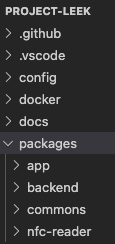
\includegraphics[width=3.8cm]{PackageStruktur.png}
  \caption{Orderstruktur}
  \label{fig:Orderstruktur}
\end{wrapfigure}
Die an das Projekt gesetzten Anforderungen machten die Erstellung mehrerer Applikationen notwendig. Neben einer Benutzeroberfläche, auf der die NFC-Tags
verwaltet werden können, musste die Steuerung des NFC-Readers und ein System zur Speicherung der Daten sowie zum Abspielen der Musik entwickelt werden.
Die dafür benötigten Anwendungen wurden als Microservices konzipiert und umgesetzt. Zur Verringerung des Aufwands der Konfiguration und Wartung wurden die einzelnen Microservices in einem Mono-Repository auf GitHub zusammengefasst.
Jeder Service wurde in einem Unterdner in \textit{packages} angelegt (vgl. Abbildung \ref{fig:Orderstruktur}). Der Ordner \textit{app} enthält die Benutzeroberfläche,
\textit{backed} die Datenbankschnittstelle sowie Logik zur Kommunikation mit dem Musik-Streaming-Anbieter und \textit{nfc-reader} die Applikation zum Steuern und auslesen des am Raspberry Pi angeschlossenen NFC-Readers.
Im Ordner commons befinden sich von allen Services gemeinsam genutzte Ressourcen (wie z. B. Modell-Klassen).
Neben den einzelnen Microservices wurden ebenfalls die Dokumentationsdateien wie Setup-Guide, Benutzerdokumentation und Projektbericht im Mono-Repo im Ordner \textit{docs} abgelegt.
Auch die für den Dienst \textit{Docker} benötigten Dateien fanden in dem gleichnamigen Ordner Platz. Die Konfigurationsdateien für den \textit{ESLint} und den \textit{Typescript}-Compiler sind im Ordner \textit{config} zu finden.
Auf die Auflistung aller weiteren Dateien wird für den Moment verzichtet. Eine genaue Aufstellung ist dem \textit{GitHub-Repository}\footnote{\url{https://github.com/project-leek/project-leek}} zu entnehmen.
Durch die Zusammenfassung in ein Mono-Repository waren die einzelnen Services für jeden Entwickler jederzeit einfach erreichbar, ohne die Notwendigkeit das Repository zu wechseln.



\subsection{Technologien und Hilfsmittel}
\colorbox{red}{TODO:}Vue, vscode, devops krams, etc
Entwickelt wird mit Visual Studio Code, da es eine einfache Nutzung des Linux-Subsystems ermöglicht. \footnote{https://code.visualstudio.com/docs/remote/wsl}.

\subsection{Deployment Cycle}
\colorbox{red}{TODO:} ziehe ticket > assigne dich selbst > draft PR > wenn fertig, setzte \textit{undraft} > assigne 2 reviewer > merge master

\subsection{Probleme während der Durchführung}
\colorbox{red}{TODO:}

\section{Projekt Meilensteine}
\subsection{Meilenstein 1}
\colorbox{red}{TODO:}Kurze Einleitung, von wann bis wann ging
\subsubsection{Ziel}
\colorbox{red}{TODO:}was haben wir uns vorgenommen, was war das ziel, was wollten wir schaffen?
\subsubsection{Probleme}
\colorbox{red}{TODO:}welche prrobleme sind aufgetreten?

\subsubsection{Lösungen}
\colorbox{red}{TODO:}Welche Lösungen haben wir gefunden?

\subsubsection{Product Increment}
\colorbox{red}{TODO:}Was ist am Ende dabei rumgekommen?

\subsubsection{Retrospektive}
\colorbox{red}{TODO:}Was haben wir dabei gelernt? Neue Erkentnisse? Neue Sichtweisen?
Was lief gut, neu gelernt, was lief nicht so gut, was verbessern?
\begin{comment}{

Lief Gut
- Zusammenarbeit und Team Environment
- Meetings und Zusammenarbeit
- Github Workflow
- Anton!!!
- Richtig viel gelernt.
- Sau viel Zeit Einsatz von Anton, muss man mal wertschätzen.
- gruppenklima
- Die Kommunikation war klasse, genauso Teamwork.

Neu Gelernt
- Vue
- Feathers
- Tailwind
- CI
- undefined & null
- feathers
- vue
- Code / PR Review

Nicht so gut
- globale Probleme waren meh
- bei Problemen (nicht weitergekommen) nicht sofort bescheid sagen
- Wörtlicher Kundenwunsch wurde viel zu spät in dem sprint behandelt. Auch wenn hello wolrd cool war müssen wir vielleicht in dem nächsten sprint härter priorisieren.

Verbessern
- Aufgabenaufteilung
- Code reviews häufiger machen
- Aufgaben früher
- Teils lange Wartezeiten
- mehr den aktuellen stand kommunizieren
- Pünktlichkeit und rumorganisation der stand ups.
}

\subsection{Meilenstein 2}
\colorbox{red}{TODO:}Kurze Einleitung,  von wann bis wann ging}
\subsubsection{Ziel}
\colorbox{red}{TODO:}was haben wir uns vorgenommen, was war das ziel, was wollten wir schaffen?}
\subsubsection{Probleme}
\colorbox{red}{TODO:}welche prrobleme sind aufgetreten?}

\subsubsection{Lösungen}
\colorbox{red}{TODO:}Welche Lösungen haben wir gefunden?}

\subsubsection{Product Increment}
\colorbox{red}{TODO:}Was ist am Ende dabei rumgekommen?}

\subsubsection{Retrospektive}
\colorbox{red}{TODO:}Was haben wir dabei gelernt? Neue Erkentnisse? Neue Sichtweisen?
Was lief gut, neu gelernt, was lief nicht so gut, was verbessern?}
\colorbox{red}{TODO:}
  Gut
- Pair Programming
- (github) workflow
- team arbeit
- Gegenseitige Hilfe
- Workflow lief besser

gelernt
- Viel Technisches (Feathers, Hooks, OAuth)
- manchmal weniger komplex denken und mehr an konkreten Problemen arbeiten
- Latex

nicht so gut
- abhängigkeiten von tickets (zumindest augenscheinlich, manchmal ist das gar nicht so der fall)
- Alles zu sehr gefühlt voneinander noch dependant, dass manche länger mal auf andere Sachen warten müssen

Verbessern
- Früher nachfragen
- probleme direkter ansprechen
- mehr pair-programming
- Presentation besser vorbereiten und vorher durchgehen
- in Daily: Cooolen Code vorstellen
- Definition-of-Done erstellen
- letzter Punkt, sollte sich aber von selber lösen
\end{comment}

\subsection{Meilenstein 3}
\colorbox{red}{TODO:}Kurze Einleitung,  von wann bis wann ging
\subsubsection{Ziel}
\colorbox{red}{TODO:}was haben wir uns vorgenommen, was war das ziel, was wollten wir schaffen?
\subsubsection{Probleme}
\colorbox{red}{TODO:}welche prrobleme sind aufgetreten?

\subsubsection{Lösungen}
\colorbox{red}{TODO:}Welche Lösungen haben wir gefunden?

\subsubsection{Product Increment}
\colorbox{red}{TODO:}Was ist am Ende dabei rumgekommen?

\subsubsection{Retrospektive}
\colorbox{red}{TODO:}Was haben wir dabei gelernt? Neue Erkentnisse? Neue Sichtweisen?
Was lief gut, neu gelernt, was lief nicht so gut, was verbessern?
\begin{comment}{
Lief Gut
- gemeinsames synchrones Arbeiten (gegen Ende)
- Teamreview
- ehrliches Miteinander
- Trotz Komplikationen und Probleme am Ende ein schönes Product Increment abgeliefert.
- Team Review hat gefühlt auch die Spannung gelöst und war sehr gut ehrlich zueinander zu sein.
- Pull Requests eindeutiger beschrieben ausgeführt (Mit Beispielen)
- Reviews schneller gemacht
- Feedback im Team
- Wichtige neue Features fertig gestellt (UI-components, Welcome Screen, Home Screen, Add-Tag Screen)
- Teamtreffen

Neu Gelernt
- stabiles Wissen mit vue (vor allem reactivity, events und components)
- Vue Parent/Child Kommunikation.
- Ein bisschen TailwindCSS.
- Neuer Vue Krams (inject & provide)
- Vue inject & provide
- Vue Prototypes
- Raspi comitup (hotspot zum WLan einrichten)


Nicht so gut
- scope des milestones: zu viele Sachen
- seeehr knappes sprintende
- Umplanung gegen Ende des Sprints
- Kommunikation und Absprache.
- Zeitmanagement.
- Fokus, was wir wirklich erledigen, was ist wichtig, was muss mindestens da sein und haben wir noch genug Zeit.
- Eingesetzte Zeit und Aufwand
- Wenig getestete Features
- Zu wenig Kommunikation zwischen den einzelnen Tickets bei Abhängigkeiten
- Meine Technik
- Zeit für Milestone / Sprint über Weihnachten & Neujahr zu lang

Verbessern
- besser abstimmmen was im Sprint gemacht werden soll
- nicht nur 'ja machen wir mal das hier alles'
- rechtzeitiger fragen bei Problemen
- Einen Tag vorher fertig mindestens
- reviews rechtzeitiger '^^
- Bessere Kommunikation und Absprache damit Ziele und Ansprüche klarer sind.
- Auch (inspiriert durch Julian) mehr "Gemeinsam lösen wir das Problem" Mindset anstelle "Wieso hast du das und das nicht gemacht?" Blameset.
- Insgesamt positiveres Mindset, denn wir schaffen ja doch schon viel.
- Zum vorletzten Daily die letzten Fixes ansprechen, dass am letzten Daily eigentlich nichts mehr ansteht.
- Fertig bis zum Vortag des nächsten Reviews
- Püntlicher zu Meetings erscheinen (Ich selbst)
- Kürzere Deadlines
- Ziele wiederholen in Meetings / klar festlegen: Was wird vom wem bis wann gemacht.
- Reviews schneller machen
- Aufgaben in kleinere Aufgaben teilen
- Zwischenstände zeigen lassen bei längeren Aufgaben
\end{comment}

\subsection{Meilenstein 4}
\colorbox{red}{TODO:}Kurze Einleitung, von, bis
\subsubsection{Ziel}
\colorbox{red}{TODO:}was haben wir uns vorgenommen, was war das ziel, was wollten wir schaffen?
\subsubsection{Probleme}
\colorbox{red}{TODO:}welche prrobleme sind aufgetreten?

\subsubsection{Lösungen}
\colorbox{red}{TODO:}Welche Lösungen haben wir gefunden?

\subsubsection{Erkenntnisse}
\colorbox{red}{Was haben wir dabei gelernt? Neue Erkentnisse? Neue Sichtweisen?}

\subsubsection{Product Increment}
\colorbox{red}{TODO:}Was ist am Ende dabei rumgekommen?

\subsubsection{Retrospektive}
\colorbox{red}{TODO:}Was haben wir dabei gelernt? Neue Erkentnisse? Neue Sichtweisen?
Was lief gut, neu gelernt, was lief nicht so gut, was verbessern?

\section{Erkenntnisse}

\section{Code Walkthrough}
\colorbox{red}{TODO:}vielleicht interessante Code Snippets?

\section{Testing}
\colorbox{red}{TODO:}wie haben wir getestet, haben wir getestet?

\section{Technische Diagramme}
\colorbox{red}{TODO:}ER Diagramme, UML, solcher krams

\newpage
\section{Anhang}
\colorbox{red}{BEISPIEL, DELETE THIS} Buchreferenz \cite{Literaturbeispiel:tom} oder Seitenref \cite{google}
\printbibliography
\end{document}
